We want to find methods for finding the particular integral of forced second order ODEs.
\subsection{Guesswork}
Here, \(f(x)\) is the forcing term.

\begin{tabular}{c c}
	Form of \(f(x)\)                        & Form of \(y_p(x)\)                          \\\midrule
	\(e^{mx}\)                              & \(Ae^{mx}\)                                 \\
	\(\sin(kx)\) or \(\cos(kx)\)            & \(A\sin(kx) + B\cos(kx)\)                   \\
	\(x^n\) or an \(n\)th degree polynomial & \(a_n x^n + a_{n-1}x^{n-1} + \cdots + a_0\)
\end{tabular}

In general:
\begin{enumerate}
	\item Insert our guess into the equation;
	\item Equate coefficients of functions;
	\item Solve for unknown coefficients.
\end{enumerate}

\subsection{Variation of parameters}
This is a method for finding the particular integral \(y_p\) given complementary functions \(y_1\), \(y_2\), which are assumed to be linearly independent, with solution vectors
\[
	\vb Y_1 = \begin{pmatrix}
		y_1 \\ y_1'
	\end{pmatrix};\quad \vb Y_2 = \begin{pmatrix}
		y_2 \\ y_2'
	\end{pmatrix}
\]
Suppose that the solution vector for \(y_p\) satisfies
\begin{equation}\label{varparam1}
	\vb Y_p = \begin{pmatrix}
		y_p \\ y_p'
	\end{pmatrix} = u(x)\vb Y_1 + v(x)\vb Y_2
\end{equation}
This is not a linear combination of \(\vb Y_1\) and \(\vb Y_2\), but we can treat it as a linear combination at a fixed \(x\) point (just as a way to visualise it).
We want to find equations for \(u(x)\) and \(v(x)\).
By comparing components of the vectors on the left and right, we have
\begin{align*}
	y_p  & = uy_1 + vy_2 \tag{a}   \\
	y_p' & = uy_1' + vy_2' \tag{b} \\
\end{align*}
So therefore,
\[
	\frac{\dd}{\dd{x}}(\mathrm a) \implies y_p' = u'y_1 + uy_1' + v'y_2 + vy_2' \tag{c}
\]
\[
	(\mathrm c) - (\mathrm b) \implies u'y_1 + v'y_2 = 0 \tag{d}
\]
Now:
\[
	\frac{\dd}{\dd{x}}(\mathrm b) \implies y_p'' = uy_1'' + u'y_1' + v'y_2' + vy_2'' \tag{e}
\]
If \(y_p'' + p(x)y_p' + q(x)y_p = f(x)\), then
\[
	(\mathrm e) + p(\mathrm b) + q(\mathrm a) = f(x)
\]
But also, \(y_1\) and \(y_2\) satisfy the differential equation
\[
	y_c'' + py_c' + qy_c = 0\quad y_c \in \{ y_1, y_2 \}
\]
After we substitute in and cancel a lot of terms, we have
\[
	u'y_1' + v'y_2' = f(x) \tag{f}
\]
Combining (d) and (f), we can deduce \(u\) and \(v\).
\[
	\underbrace{\begin{pmatrix}
			y_1 & y_2 \\ y_1' & y_2'
		\end{pmatrix}}_{\mathclap{\text{fundamental matrix}}} \begin{pmatrix}
		u' \\ v'
	\end{pmatrix} = \begin{pmatrix}
		0 \\ f
	\end{pmatrix}
\]
So as long as \(y_1\) and \(y_2\) are linearly independent, i.e.\ the Wro\'nskian is nonzero, we can write an equation for \(u'\) and \(v'\).
\[
	\begin{pmatrix}
		u' \\ v'
	\end{pmatrix} = \frac{1}{W(x)}\begin{pmatrix}
		y_2' & -y_2 \\ y_1' & y_1
	\end{pmatrix} \begin{pmatrix}
		0 \\ f
	\end{pmatrix}
\]
or explicitly,
\begin{align*}
	u' & = \frac{-y_2 f}{W} \\
	v' & = \frac{y_1 f}{W}
\end{align*}
and therefore
\[
	y_p = y_2 \int^x \frac{y_1(t) f(t)}{W(t)}\dd{t} - y_1 \int^x \frac{y_2(t) f(t)}{W(t)}\dd{t}
\]

\subsection{Forced oscillating systems: transients and damping}
Many physical systems have a restoring force and damping (e.g.
friction).
For example, the suspension of a car could be modelled with \(y(t)\), where \(y\) is the height of the wheel, given by
\[
	M\ddot y = F(t) - \underbrace{ky}_{\text{spring}} - \underbrace{L\dot y}_{\text{damper}}
\]
In standard form, we have
\[
	\ddot y + \frac{L}{M} \dot y + \frac{k}{M} y = \frac{F(t)}{M}
\]
Let \(\tau = \sqrt{\frac{k}{M}} t\).
Then we can rewrite this equation using a single parameter:
\[
	y'' + 2Ky' + y = f(\tau)
\]
where \(y' = \frac{\dd{y}}{\dd \tau}\), \(K = \frac{L}{2\sqrt{kM}}\), \(f = \frac{F}{k}\).
Our unforced system is described here by one parameter \(K\).

In the case of the unforced response (also known as the free or natural response), we have \(f=0\), so
\[
	y'' + 2Ky' + y = 0
\]
Solving by the characteristic equation, we see
\[
	\lambda = -K \pm \sqrt{K^2 - 1}
\]
There are a number of cases here.
\begin{enumerate}
	\item (\(K < 1\)) This produces a decaying oscillation, known as `underdamped'.
	      \(\lambda_1, \lambda_2\) are both complex, and therefore
	      \[
		      y = e^{-K\tau}\left[A\sin(\sqrt{1-K^2}\tau) + B\cos(\sqrt{1-K^2}\tau)\right]
	      \]
	      The period is \(\frac{2\pi}{\sqrt{1-K^2}}\).
	      As \(K\) tends to 1, the period tends to \(\infty\).
	\item (\(K = 1\)) This is the degenerate case, \(\lambda_1 = \lambda_2 = -K\).
	      We can use detuning to deduce
	      \[
		      y = e^{-K\tau} (A + B\tau)
	      \]
	\item (\(K > 1\)) Here, we have two negative real roots \(\lambda_1, \lambda_2\); this situation is known as `overdamped'.
	      \[
		      y = Ae^{\lambda_1 \tau} + Be^{\lambda_2 \tau}
	      \]
\end{enumerate}
Note that the unforced response decays in all cases.

\subsection{Sinusoidal forcing}
Let
\[
	\ddot y + \mu \dot y + \omega_0^2 y = \sin \omega t
\]
Now let us guess \(y_p = A\sin \omega t + B\cos \omega t\).
Equating coefficients of \(\sin\omega t\) gives
\[
	-A\omega^2 - B\mu\omega + \omega_0^2A = 1 \tag{a}
\]
and equating \(\cos\omega t\) gives
\[
	-B\omega^2 + A\mu\omega + \omega_0^2B = 0 \tag{b}
\]
Then:
\[
	(\text b) \implies A = B \frac{\omega^2 - \omega_0^2}{\mu\omega}
\]
\[
	(\text a) \implies A(\omega_0^2 - \omega^2) = 1 + B\mu\omega
\]
So
\[
	A = \frac{\omega_0^2 - \omega^2}{(\omega_0^2 - \omega^2)^2 + \mu^2\omega^2}
\]
\[
	B = \frac{-\mu\omega}{(\omega_0^2 - \omega^2)^2 + \mu^2\omega^2}
\]
Altogether, we have
\[
	y_p = \frac{1}{(\omega_0^2 - \omega^2)^2 + \mu^2\omega^2}\left[ (\omega_0^2 - \omega^2)\sin\omega t - \mu \omega \cos \omega t \right]
\]
Drawing an example of this kind of particular integral in red (with the complementary function in blue), we can see the following:

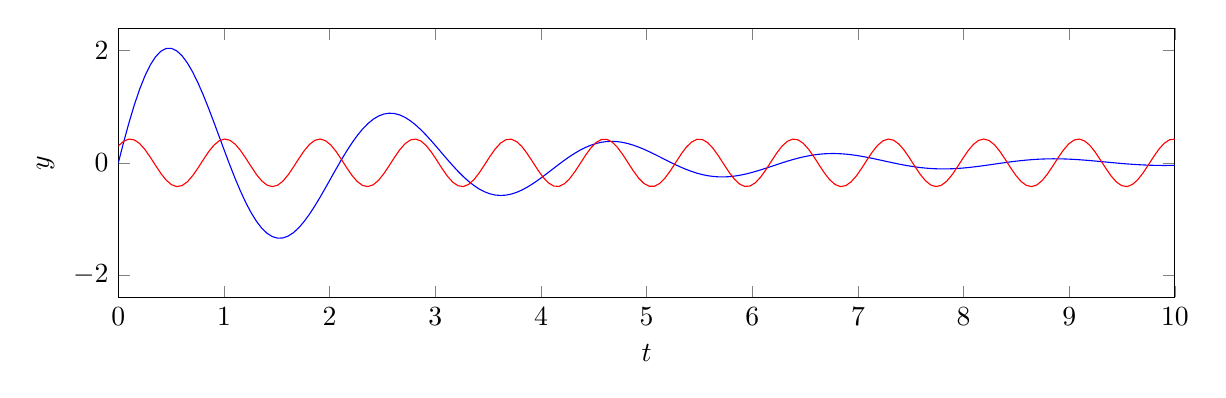
\begin{tikzpicture}
	\begin{axis}[
			%axis lines = left,
			xlabel = \(t\),
			ylabel = \(y\),% \(y = y_c + y_p\),
			width=15cm,
			height=5cm,
			xmin=0,
			xmax=10,
			ymin=-2.4,
			ymax=2.4
			%xticklabel=\empty,
			%yticklabel=\empty
		]

		\addplot [
			domain=0:10,
			samples=200,
			color=blue
		]
		{2.5*e^(-0.4*x)*sin(3*deg(x))};

		\addplot [
			domain=0:10,
			samples=200,
			color=red
		]
		{0.3*(sin(7*deg(x)) + cos(7*deg(x)))};
	\end{axis}
\end{tikzpicture}

And adding both together to form a particular solution gives:

\begin{tikzpicture}
	\begin{axis}[
			%axis lines = left,
			xlabel = \(t\),
			ylabel = \(y\),% \(y = y_c + y_p\),
			width=15cm,
			height=5cm,
			xmin=0,
			xmax=10,
			ymin=-2.4,
			ymax=2.4
			%xticklabel=\empty,
			%yticklabel=\empty
		]

		\addplot [
			domain=0:10,
			samples=200,
			color=black
		]
		{2.5*e^(-0.4*x)*sin(3*deg(x)) + 0.3*(sin(7*deg(x)) + cos(7*deg(x)))};
	\end{axis}
\end{tikzpicture}

Let us make a few comments about these forced oscillations.
\begin{itemize}
	\item The complementary function gives us the transient (short-term) response to the initial conditions.
	\item The particular integral gives the long-term response to the forcing term.
	\item In some sense, the system `forgets' about the initial conditions over time due to the damping term.
\end{itemize}

\subsection{Resonance in undamped systems}
What happens if \(\omega = \omega_0\)?
If \(\mu \neq 0\) (i.e.\ it is a damped system), then
\[
	\lim_{\omega \to \omega_0} y_p = \frac{-\cos\omega_0 t}{\mu\omega_0}
\]
This is a finite amplitude oscillation.
Note that the amplitude increases with decreasing \(\mu\), so clearly this solution has a problem at \(\mu = 0\).
To work with this, we'll let
\[
	\ddot y + \omega_0^2 y = \sin\omega_0 t
\]
We will use detuning to get solutions for this equation.
Consider instead
\[
	\ddot y + \omega_0^2 y = \sin\omega t
\]
where \(\omega \neq \omega_0\).
We will guess that the particular integral is of the form \(y_p = C\sin\omega t\) since by inspection there cannot be any cosine terms.
\[
	C(-\omega^2 + \omega_0^2) = 1
\]
\[
	\therefore y_p = \frac{1}{\omega_0^2 - \omega^2}\sin\omega t
\]
As the system is linear in \(y\) and its derivatives, we can freely add some multiple of the complementary function and it will remain a solution.
\[
	y_p = \frac{1}{\omega_0^2 - \omega^2}\sin\omega t + A \sin\omega_0 t
\]
Now let us pick \(A = \frac{-1}{\omega_0^2 - \omega^2}\), so
\[
	y_p = \frac{\sin \omega t - \sin \omega_0 t}{\omega_0^2 - \omega^2}
\]
Rewriting this using angle addition and subtraction identities:
\[
	y_p = \frac{2}{\omega_0^2 - \omega^2}\left[ \cos\left( \frac{\omega + \omega_0}{2}t \right) \sin\left( \frac{\omega - \omega_0}{2}t \right) \right]
\]
For convenience, let \(\Delta\omega \equiv \omega_0 - \omega\), and therefore \(\frac{\omega + \omega_0}{2} = w_0 - \frac{1}{2}\Delta\omega\).
\[
	y_p = \frac{-2}{\Delta\omega(\omega_0 + \omega)}\left[ \cos\left( \left(\omega_0 - \frac{\Delta\omega}{2}\right)t \right) \sin\frac{\Delta\omega t}{2} \right]
\]
In the following diagram, \(y_p\) is drawn in blue, with the sine term (in red) acting as an envelope for the higher-frequency cosine term.
The phenomenon visible here is known as `beating', as an oscillator with a fundamental frequency slightly different to the forcing frequency will begin oscillating then stop, and repeat this cycle.

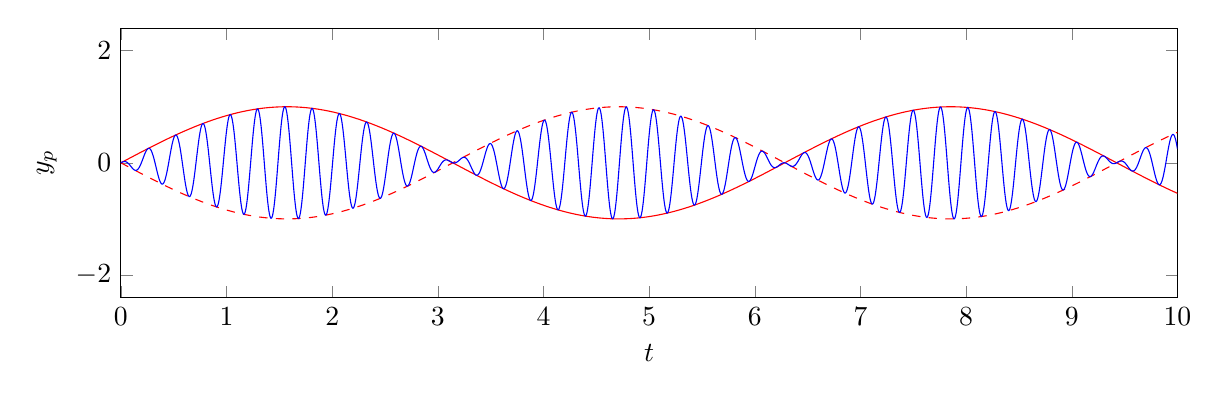
\begin{tikzpicture}
	\begin{axis}[
			%axis lines = left,
			xlabel = \(t\),
			ylabel = \(y_p\),% \(y = y_c + y_p\),
			width=15cm,
			height=5cm,
			xmin=0,
			xmax=10,
			ymin=-2.4,
			ymax=2.4
			%xticklabel=\empty,
			%yticklabel=\empty
		]

		\addplot [
			domain=0:10,
			samples=200,
			color=red
		]
		{sin(deg(x))};
		\addplot [
			dashed,
			domain=0:10,
			samples=200,
			color=red
		]
		{-sin(deg(x))};

		\addplot [
			domain=0:10,
			samples=2000,
			color=blue
		]
		{cos(24.3*deg(x))*sin(deg(x))};
	\end{axis}
\end{tikzpicture}

As we reduce \(\Delta\omega\) to zero, we have
\[
	\lim_{\Delta\omega\to 0} \sin\left(\frac{\Delta\omega}{2}t\right) \approx \frac{\Delta\omega}{2}t
\]
So
\begin{align*}
	\lim_{\Delta\omega\to 0}
	 & \approx \frac{-2}{\Delta\omega(\omega_0 + \omega_0)} \cos(\omega_0t)\left(\frac{\Delta\omega}{2}t\right) \\
	 & \approx \frac{-2t}{\omega_0} \cos\omega_0t                                                               \\
\end{align*}
This is linear growth in amplitude over time.
This increase is unbounded an in undamped system.
Note that \(y_p\) takes the form of one of the complementary functions multiplied by the independent variable.

\subsection{Impulses and point forces}
Consider a system that experiences a sudden force, for example a car's suspension when driving over a speed bump.
Let us define \(y\) to be the displacement from the undisturbed height of the suspension.
Let the car's mass be \(M\).
In a small finite window \(\varepsilon\) around some time \(T\), the excess force \(F\) (the forcing term) on the system is greater than zero.
As \(\varepsilon\) tends to zero, the force becomes a sudden impulse.
Let us model this using the equation
\[
	M\ddot y = F(t) - ky - L\dot y
\]
We can see that before time \(T\), \(y=0\).
After this point, there is some kind of oscillation.
Note that the value of \(y\) is always continuous (otherwise this would violate many laws of physics), but the derivative is not necessarily continuous at the point \(T\).
Let us integrate the equation above in time from \(T - \varepsilon\) to \(T + \varepsilon\).
\begin{equation}\label{impulse1}
	\lim_{\varepsilon \to 0} \left[ M[\dot y]_{T - \varepsilon}^{T + \varepsilon} = \int_{T - \varepsilon}^{T + \varepsilon} F(t) \dd{t} - k \underbrace{\int_{T - \varepsilon}^{T + \varepsilon} y \dd{t}}_{0\text{ if \(y\) is finite}} - L\underbrace{[y]_{T - \varepsilon}^{T + \varepsilon}}_{0\text{ if \(y\) is continuous}} \right]
\end{equation}
We now can define the impulse \(I\) to be
\[
	I = \lim_{\varepsilon \to 0} \int_{T - \varepsilon}^{T + \varepsilon} F(t) \dd{t}
\]
Hence
\[
	\eqref{impulse1} \implies I = \lim_{\varepsilon \to 0} M[\dot y]_{T - \varepsilon}^{T + \varepsilon}
\]
So if the impulse is nonzero, the velocity \(\dot y\) experiences a sudden change, so it is discontinuous at \(T\).
The value of this sudden change in velocity depends on the integral of the force.
